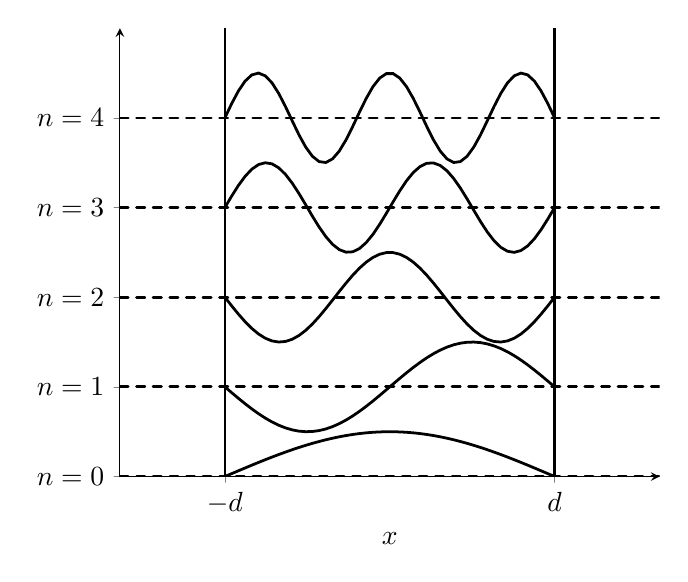
\begin{tikzpicture}[cap=round,>=latex]
\begin{axis}[grid=none,
axis x line=bottom,
axis y line=left,	
%enlargelimits,
xtick={0,3.1415},
xticklabels={$-d$, $d$},
ytick={0,2,4,6,8},
yticklabels={$n = 0$,$n = 1$, $n = 2$, $n = 3$, $n = 4$},
xlabel={$x$},
xmin=-1,
xmax=pi+1,
ymin=0,
ymax=10,
]

%sym 0
\addplot[no markers, line width=1, samples=50, domain=0:pi] {cos(deg(x-pi/2))};

%\addplot[no markers, line width=1, samples=50, domain=-1:0.3]{exp(x)*(cos(deg(0.3-pi/2)))+0.5};
%\addplot[no markers, line width=1, samples=50, domain=pi-0.3:pi+1]{exp(-x+pi-0.3)*(cos(deg(pi-0.3))+0.5)};
\addplot[no markers, dashed, line width=1, samples=50, domain=-1:pi+1]{0};

%antisym 1
\addplot[no markers, line width=1, samples=50, domain=0:pi] {sin(deg(2*(x-pi/2)))+2};
\addplot[no markers, dashed, line width=1, samples=50, domain=-1:pi+1]{2};

%sym 2
\addplot[no markers, line width=1, samples=50, domain=0:pi] {cos(deg(3*(x-pi/2)))+4};
\addplot[no markers, dashed, line width=1, samples=50, domain=-1:pi+1]{4};

%antisym 3
\addplot[no markers, line width=1, samples=50, domain=0:pi] {sin(deg(4*(x-pi/2)))+6};
\addplot[no markers, dashed, line width=1, samples=50, domain=-1:pi+1]{6};

%sym 2
\addplot[no markers, line width=1, samples=50, domain=0:pi] {cos(deg(5*(x-pi/2)))+8};
\addplot[no markers, dashed, line width=1, samples=50, domain=-1:pi+1]{8};

\addplot [no markers, line width=1] coordinates {(0, 0) (0, 10)};
\addplot [no markers, line width=1] coordinates {(pi, 0) (pi, 10)};
\end{axis}								


\end{tikzpicture}
